\documentclass{article}
\usepackage[landscape, margin=1cm]{geometry}
\usepackage{tikz}
\usepackage{xcolor}
\usepackage{caption}
\usepackage{pgfplots}
\pgfplotsset{compat=1.16}

\begin{document}

\begin{center}
  \huge Aircraft Boarding Strategy Comparison\\
  \Large Visualization and Performance Analysis
\end{center}

\begin{figure}[ht]
  \centering
  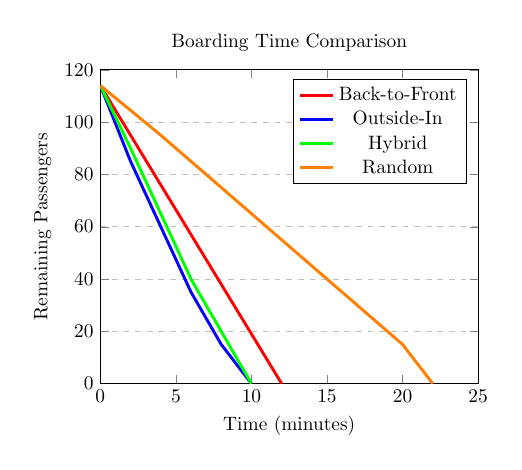
\begin{tikzpicture}[scale=0.7]
    \begin{axis}[
      title={Boarding Time Comparison},
      xlabel={Time (minutes)},
      ylabel={Remaining Passengers},
      xmin=0, xmax=25,
      ymin=0, ymax=120,
      legend pos=north east,
      ymajorgrids=true,
      grid style=dashed,
    ]
    
    % Back-to-Front strategy
    \addplot[
      color=red,
      mark=none,
      line width=1.5pt,
    ] coordinates {
      (0,114)(2,95)(4,76)(6,57)(8,38)(10,19)(12,0)
    };
    
    % Outside-In strategy
    \addplot[
      color=blue,
      mark=none,
      line width=1.5pt,
    ] coordinates {
      (0,114)(2,85)(4,60)(6,35)(8,15)(10,0)
    };
    
    % Hybrid strategy
    \addplot[
      color=green,
      mark=none,
      line width=1.5pt,
    ] coordinates {
      (0,114)(2,90)(4,65)(6,40)(8,20)(10,0)
    };
    
    % Random strategy
    \addplot[
      color=orange,
      mark=none,
      line width=1.5pt,
    ] coordinates {
      (0,114)(4,95)(8,75)(12,55)(16,35)(20,15)(22,0)
    };
    
    \legend{Back-to-Front, Outside-In, Hybrid, Random}
    
    \end{axis}
  \end{tikzpicture}
  \caption{Comparison of passenger boarding times across different strategies}
  \label{fig:time-comparison}
\end{figure}

\begin{center}
  \Large Boarding Strategy Visualizations
\end{center}

\begin{figure}[ht]
  \centering
  \begin{tikzpicture}[scale=0.55]
    % Back-to-Front
    \begin{scope}[xshift=0cm]
      \node[font=\bfseries] at (3, 1) {Back-to-Front};
      
      % Seat grid
      \foreach \r in {1,...,6}{
        \foreach \c in {1,...,6}{
          % Color by zone (back to front)
          \ifnum\r<3
            \fill[blue!70] (\c-1,-\r) rectangle ++(1,-1);
          \else
            \ifnum\r<5
              \fill[blue!40] (\c-1,-\r) rectangle ++(1,-1);
            \else
              \fill[blue!20] (\c-1,-\r) rectangle ++(1,-1);
            \fi
          \fi
          \draw[thick] (\c-1,-\r) rectangle ++(1,-1);
        }
      }
      
      % Aisle
      \draw[dashed, thick] (3, 0) -- (3, -7);
      
      % Time
      \node at (3, -7.5) {12 min};
    \end{scope}
    
    % Outside-In
    \begin{scope}[xshift=8cm]
      \node[font=\bfseries] at (3, 1) {Outside-In};
      
      % Seat grid
      \foreach \r in {1,...,6}{
        \foreach \c in {1,...,6}{
          % Color by seat position (window, middle, aisle)
          \ifnum\c=1
            \fill[green!70] (\c-1,-\r) rectangle ++(1,-1);
          \else
            \ifnum\c=6
              \fill[green!70] (\c-1,-\r) rectangle ++(1,-1);
            \else
              \ifnum\c=2
                \fill[green!40] (\c-1,-\r) rectangle ++(1,-1);
              \else
                \ifnum\c=5
                  \fill[green!40] (\c-1,-\r) rectangle ++(1,-1);
                \else
                  \fill[green!20] (\c-1,-\r) rectangle ++(1,-1);
                \fi
              \fi
            \fi
          \fi
          \draw[thick] (\c-1,-\r) rectangle ++(1,-1);
        }
      }
      
      % Aisle
      \draw[dashed, thick] (3, 0) -- (3, -7);
      
      % Time
      \node at (3, -7.5) {10 min};
    \end{scope}
    
    % Hybrid
    \begin{scope}[xshift=16cm]
      \node[font=\bfseries] at (3, 1) {Hybrid};
      
      % Seat grid
      \foreach \r in {1,...,6}{
        \foreach \c in {1,...,6}{
          % Zone factor
          \pgfmathtruncatemacro{\zone}{0}
          \ifnum\r<3
            \pgfmathtruncatemacro{\zone}{3} % Back zone
          \else
            \ifnum\r<5
              \pgfmathtruncatemacro{\zone}{2} % Middle zone
            \else
              \pgfmathtruncatemacro{\zone}{1} % Front zone
            \fi
          \fi
          
          % Seat type factor
          \pgfmathtruncatemacro{\type}{0}
          \ifnum\c=1
            \pgfmathtruncatemacro{\type}{3} % Window
          \else
            \ifnum\c=6
              \pgfmathtruncatemacro{\type}{3} % Window
            \else
              \ifnum\c=2
                \pgfmathtruncatemacro{\type}{2} % Middle
              \else
                \ifnum\c=5
                  \pgfmathtruncatemacro{\type}{2} % Middle
                \else
                  \pgfmathtruncatemacro{\type}{1} % Aisle
                \fi
              \fi
            \fi
          \fi
          
          % Combined priority (higher is earlier)
          \pgfmathtruncatemacro{\priority}{\zone+\type}
          \pgfmathsetmacro{\colorintensity}{\priority*10}
          
          \fill[red!\colorintensity] (\c-1,-\r) rectangle ++(1,-1);
          \draw[thick] (\c-1,-\r) rectangle ++(1,-1);
        }
      }
      
      % Aisle
      \draw[dashed, thick] (3, 0) -- (3, -7);
      
      % Time
      \node at (3, -7.5) {10 min};
    \end{scope}
    
    % Random
    \begin{scope}[xshift=24cm]
      \node[font=\bfseries] at (3, 1) {Random};
      
      % Random pattern
      \foreach \r in {1,...,6}{
        \foreach \c in {1,...,6}{
          % Use fixed "random" pattern for illustration
          \pgfmathtruncatemacro{\rand}{(\r*\c*13) % 100}
          \fill[orange!\rand] (\c-1,-\r) rectangle ++(1,-1);
          \draw[thick] (\c-1,-\r) rectangle ++(1,-1);
        }
      }
      
      % Aisle
      \draw[dashed, thick] (3, 0) -- (3, -7);
      
      % Time
      \node at (3, -7.5) {22 min};
    \end{scope}
    
  \end{tikzpicture}
  \caption{Visual comparison of the four boarding strategies}
  \label{fig:strategy-comparison}
\end{figure}

\begin{center}
  \Large Strategy Performance Comparison
\end{center}

\begin{tabular}{|l|p{8cm}|c|c|}
  \hline
  \textbf{Strategy} & \textbf{Description} & \textbf{Time (min)} & \textbf{Efficiency} \\
  \hline
  Back-to-Front & Passengers board in zones from the back of the aircraft to the front & 12 & 54\% \\
  \hline
  Outside-In & Passengers board based on seat position (window → middle → aisle) & 10 & 65\% \\
  \hline
  Hybrid & Combination of outside-in and back-to-front approaches & 10 & 65\% \\
  \hline
  Random & No organization, passengers board in random order & 22 & 30\% \\
  \hline
\end{tabular}

\begin{center}
  \Large Key Findings from the Research
\end{center}

\begin{itemize}
  \item The traditional back-to-front strategy is not the most efficient method
  \item Outside-in boarding reduces in-row interference, a major cause of boarding delays
  \item Hybrid strategies can be optimized to achieve the best performance
  \item Random boarding is significantly less efficient than organized methods
  \item For a Boeing 737-800 with 114 economy seats, the time savings between the best and worst strategies is approximately 12 minutes
  \item Mathematical modeling using differential equations provides a useful framework for analyzing boarding dynamics
\end{itemize}

\end{document}